\documentclass[12pt, a4paper]{article}
\usepackage[UTF8]{ctex}
\usepackage{amsmath}
\usepackage{amssymb}
\usepackage{amsthm}
\usepackage{geometry}
\usepackage{enumitem}
\usepackage{indentfirst}
\usepackage{caption}
\usepackage{fancyhdr}
\usepackage{booktabs}
\usepackage{titlesec}
\usepackage{draftwatermark}%水印
\usepackage{graphicx} % 导入图像的宏包、单图
% 页面布局设置
\geometry{top=2.54cm, bottom=2.54cm, left=3.18cm, right=3.18cm}

\SetWatermarkText{B站：布加拉提}
\SetWatermarkScale{0.4}

% 行距设置
\linespread{1.5}

% 段落设置
\setlength{\parindent}{2em}
\setlength{\parskip}{0.5em}

% 节标题格式设置
\titleformat{\section}{\normalfont\Large\bfseries}{第\chinese{section}章、}{1em}{}
\titlespacing{\section}{0pt}{2.5ex plus 1ex minus .2ex}{1.3ex plus .2ex}

% 定理环境设置
\newtheoremstyle{solution}
{}
{}
{}
{}
{\bfseries}
{、}
{1em}
{}
\theoremstyle{solution}
\newtheorem{sol}{解}

% 页眉页脚设置
\pagestyle{fancy}
\fancyhf{}
\fancyhead[C]{b站布加拉提整理（回忆版）b站甘茶w独家讲解}
\fancyfoot[C]{\thepage}

\rfoot{整理人：八方\\资源提供：考研乔瑟夫}
\lhead{
\includegraphics[width=0.06\linewidth]{p1.png}}
\rhead{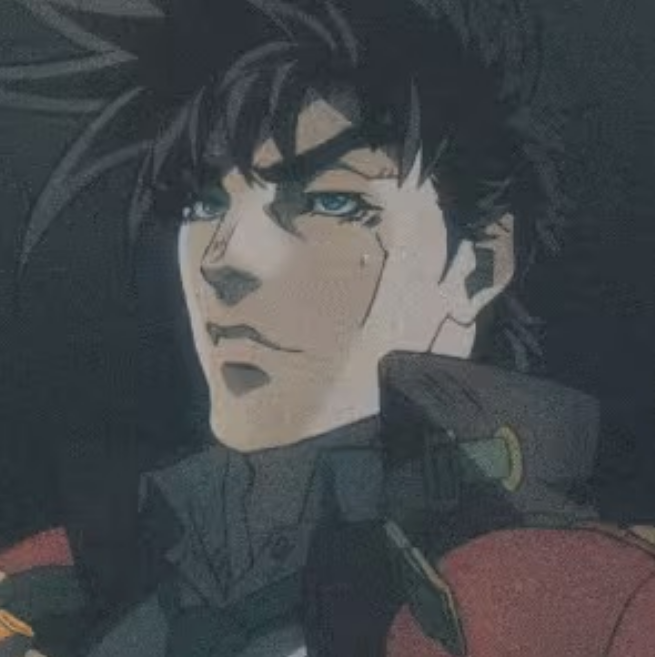
\includegraphics[width=0.06\linewidth]{p2.png}}
\renewcommand{\headrulewidth}{0.4pt}
\renewcommand{\footrulewidth}{0.4pt}

\begin{document}

\begin{center}
\Large\textbf{2015哈工大硕士考试试题：805物理光学}
\end{center}





\section*{一、填空题（20分）}
\begin{enumerate}
    \item 在迈克尔逊干涉仪实验中，测得空气层厚度变化$0.25mm$时，条纹变化了916个，求所用光的波长\_\_\_\_\_，若空气层厚度变化时，从条纹出现到再次消失总共数得条纹3500条，光源发出光波的谱线宽度是\_\_\_\_\_。
    \item 将一工件放入干涉光路中形成劈尖，观察到干涉条纹有弯曲，相邻暗纹间距为$e$，条纹最大弯曲度处与该条纹的间距为$0.8e$，若光波波长为$\lambda$,那么不平处的高度为\_\_\_\_\_，如果工件有凹陷，条纹弯曲的方向是\_\_\_\_\_劈尖。
    \item 一块波带片的孔径中有10个半波带，其中5个偶数波带被挡住，则轴上的光强比自由传播时大\_\_\_\_\_倍。
    \item 要使一束线偏振光通过偏振片后振动方向转过90度，至少需要让这束光通过\_\_\_\_\_块理想偏振片，在此情况下，最大透射光强与原来光强的比值为\_\_\_\_\_，若要用一个元件来实现，应该采用\_\_\_\_\_，其光轴与线偏振光成\_\_\_\_\_角。
    \item 点光源发出的光波在晶体中传播时，实际波面是\_\_\_\_\_法线面是\_\_\_\_\_。
    \item 采用光程概念的好处是\_\_\_\_\_。
    \item 平行平板产生的是\_\_\_\_\_干涉；楔形产生的是\_\_\_\_\_干涉。
    \item 波动的基本特征可用\_\_\_\_\_，\_\_\_\_\_和\_\_\_\_\_来描述。
\end{enumerate}
\section*{二、名词解释（18分）}
\begin{enumerate}
    \item 艾里斑
    \item 布儒斯特角
    \item 色散
    \item 巴比涅原理
    \item 半波损失
    \item 双折射
\end{enumerate}
\section*{三、选择题（18分）}
\begin{enumerate}
    \item 一个右旋圆偏振光在50度角下入射到空气-玻璃界面$(n=1.5)$，则反射光是\_\_\_\_\_。\\
    A.右旋圆偏振光 \quad B.左旋圆偏振光 \quad C.左旋椭圆偏振光 \quad D.右旋椭圆偏振光
    \item 设线数$N_1=600$的光栅其零级主级大强度为$I_1$，其他条件相同时，$N=1800$的光栅其零级主级大强度为$I_2$，则$I_1/I_2$为\_\_\_\_\_。\\
    A.1/3 \quad B.1/9 \quad C.3 \quad D.9
    \item 在闪耀光栅中，使刻槽面与光栅面成$\theta $角度，目的是\_\_\_\_\_。\\
    A.干涉条大纹与衍射零级在空间分开 \quad B.条纹变宽 \quad C.干涉条纹与衍射零级在空间重合 \quad D.自由光谱范围增
    \item 经偏振片观察部分偏振光，当偏振片由对应极大强度的位置转过60度时，光强减少为一半，则光束的偏振度为\_\_\_\_\_。\\
    A.1/3 \quad B.1/2 \quad C.1/4 \quad D.1/5
    \item 单轴晶体$e$光的折射率与$n_o,n_e$有关，除此之外还与其他相关的是\_\_\_\_\_。\\
    A.$e$光波法线与界面法线夹角\quad B.$e$光波法线与光轴夹角 \quad C.$e$光与界面法线夹角 \quad D.光线与光轴夹角
    \item 在各向异性的晶体中，光波$E$和$D$的方向\_\_\_\_\_。\\(A)一定相同\quad(B)互相垂直\quad(C)不一定相同\quad(D)一定不同
\end{enumerate}
\section*{四、简答题（30分）}
\begin{enumerate}
    \item 什么是空间相干性和时间相干性，他们是怎样产生的？
    \item 惠更斯-菲涅尔原理
    \item 什么是等相面和等幅面？举例说明二者一致和不一致的情况。
    \item 什么是空间相干性和时间相干性，他们是怎样产生的？
    \item 给定光滑的玻璃表面和金属表面，问：自然光分别在两表面上反射，是否可以获得偏振光，条件是什么？偏振光分别在两表面上，反射光的偏振性质如何？为什么？
    \item 迈克尔逊干涉仪和$F-P$干涉仪的原理属于哪一类干涉？该类干涉特点是什么？两个干涉图形有什么不同？两个干涉仪各举一个应用例子。
    \item 什么是旋光效应？法拉第磁光效应和自然旋光现象有何不同，如何利用磁致旋光效应制作单通光闸？
\end{enumerate}
\section*{五、计算与分析（41分）}
\begin{enumerate}
    \item 双星之间角距离为$1\times10^{-6}rad$，其辐射波长为$577nm$和$579nm$两个波长。问：
          \begin{enumerate}
                \item 望远镜的口径需要多大才能分辨此双星的像？
                \item 若要用一级光谱分辨此两波长，光栅条数应为多少？
          \end{enumerate}
          \begin{figure}[!htb]
                \centering
                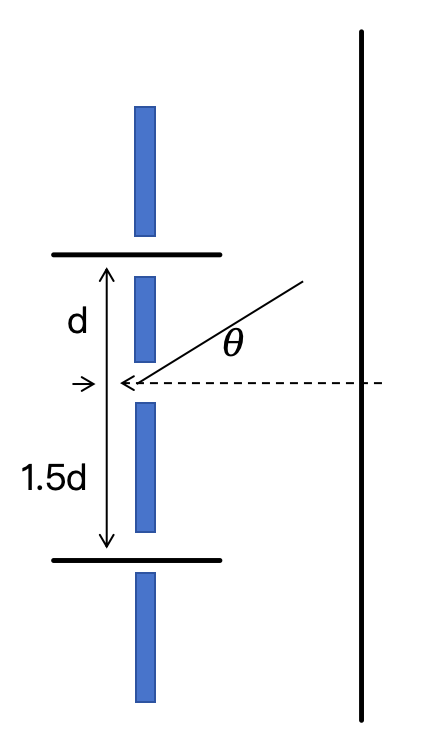
\includegraphics[width=0.4\linewidth]{151.png}              
          \end{figure}
    \item 考虑如图所示三狭缝，平行光从左侧入射，假设：三缝宽度相等$(a=6/d)$,缝距分别是$d$和$3d/2$。求衍射图样中：
          \begin{enumerate}
                \item 第一级主级大的$\theta _1$是多少？
                \item 若在$\theta =0$方向的光强为$I_0$，问在$\theta _1/2$方向的光强是多少？

    \item （重复）一个线偏振光在玻璃中传播时的表达式为：$E_x=0,E_y=0,E_z=(100V/m)(\pi\times10^{14}\times s^{-1}(t-\frac{x}{c})+\frac{\pi}{2})$,求该光的频率，波长，振幅，周期，初相位是多少？
    \item （重复）一束自然光正入射到重叠的两个偏振片上，如果透射光强为入射光强的$3/8$，求两个偏振片的夹角。
\end{enumerate}
\section*{六、论述题（10分）}
\begin{enumerate}
    \item 在焦距$200mm$和口径$90mm$的理想透镜光轴上，紧贴透镜放置一开口直径$80mm$的挡光板，分析焦平面上的光强分布。在焦屏面前放置一块折射率为$1.65$的组合棱镜（无附加像差），其他条件不变，分析焦平面上的光强分布，平面波入射，波长为$0.62um$，两种情况如下图。
         \begin{figure}[!htb]
                \centering
                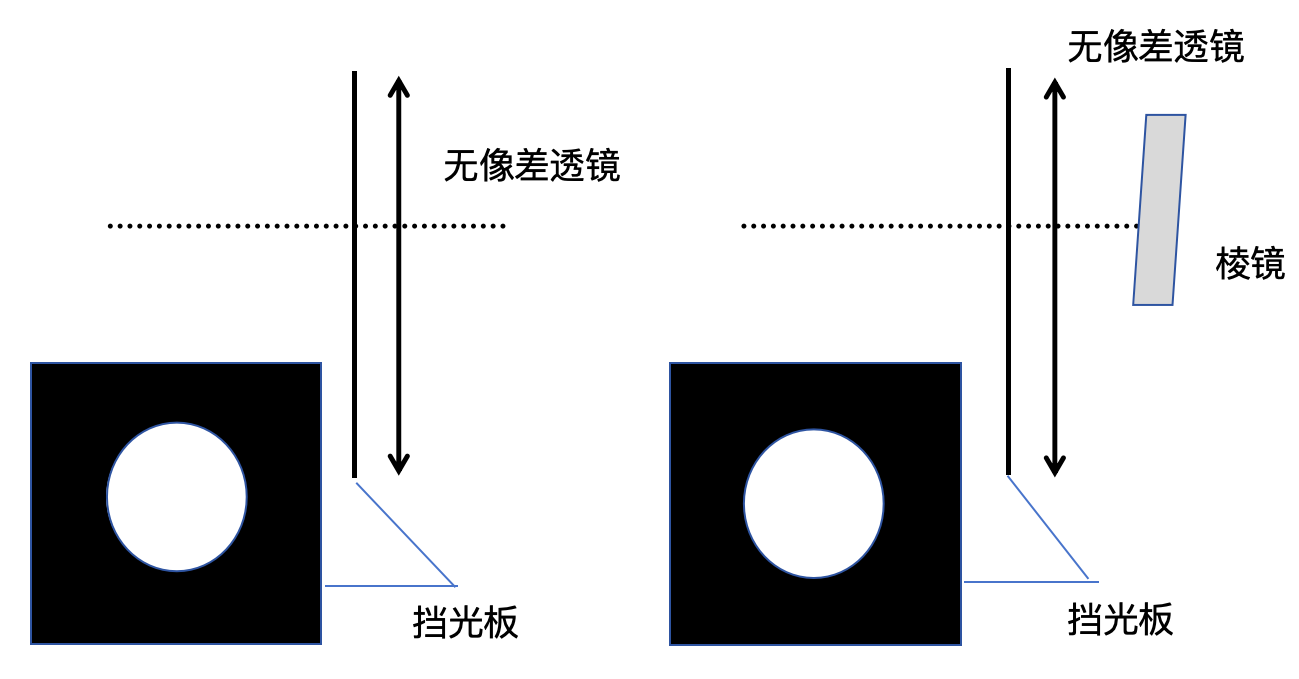
\includegraphics[width=0.7\linewidth]{152.png}
                
          \end{figure}
\end{enumerate}
\end{document}